% CVPR 2026 Paper Template; see https://github.com/cvpr-org/author-kit

\documentclass[10pt,twocolumn,letterpaper]{article}

%%%%%%%%% PAPER TYPE  - PLEASE UPDATE FOR FINAL VERSION
% \usepackage{cvpr}              % To produce the CAMERA-READY version
\usepackage[review]{cvpr}      % To produce the REVIEW version
% \usepackage[pagenumbers]{cvpr} % To force page numbers, e.g. for an arXiv version
\usepackage{multirow}
% Import additional packages in the preamble file, before hyperref

\usepackage{algorithm}
\usepackage{algpseudocode}
\input{preamble}

% It is strongly recommended to use hyperref, especially for the review version.
% hyperref with option pagebackref eases the reviewers' job.
% Please disable hyperref *only* if you encounter grave issues, 
% e.g. with the file validation for the camera-ready version.
%
% If you comment hyperref and then uncomment it, you should delete *.aux before re-running LaTeX.
% (Or just hit 'q' on the first LaTeX run, let it finish, and you should be clear).
\definecolor{cvprblue}{rgb}{0.21,0.49,0.74}
\usepackage[pagebackref,breaklinks,colorlinks,allcolors=cvprblue]{hyperref}

%%%%%%%%% PAPER ID  - PLEASE UPDATE
\def\paperID{*****} % *** Enter the Paper ID here
\def\confName{CVPR}
\def\confYear{2026}

%%%%%%%%% TITLE - PLEASE UPDATE
%\title{SpiderMark: A Hybrid Watermarking Framework for Generative AI with Algorithmic Injection and Learning Verification\\
%OR alternatively \\
\title{SpiderMark: Hybrid Watermarking for Generative AI via Algorithmic Injection and Learning-Based Verification}

%%%%%%%%% AUTHORS - PLEASE UPDATE
\author{First Author\\
Institution1\\
Institution1 address\\
{\tt\small firstauthor@i1.org}
% For a paper whose authors are all at the same institution,
% omit the following lines up until the closing ``}''.
% Additional authors and addresses can be added with ``\and'',
% just like the second author.
% To save space, use either the email address or home page, not both
\and
Second Author\\
Institution2\\
First line of institution2 address\\
{\tt\small secondauthor@i2.org}
}

\begin{document}
\maketitle
\begin{abstract}
\color{red} 
The proliferation of diffusion-based generative models has intensified the need for reliable methods to trace and verify the provenance of AI-generated images. Existing watermarking approaches for diffusion models typically rely on isotropic frequency patterns and handcrafted detection metrics, which suffer from directional vulnerability and threshold instability across diverse image transformations. We propose SpiderMark, a hybrid watermarking framework that couples algorithmic frequency-domain injection with learning-based probabilistic verification, requiring no modification to pretrained diffusion model weights. SpiderMark embeds a structured spider-web pattern, comprising radial spokes and concentric polygonal rings, into the Fourier representation of the initial latent noise, and trains a lightweight ResNet-18 verifier augmented with auxiliary similarity cues (PSNR and L1) to produce calibrated confidence scores for watermark detection. Extensive experiments across nine image transformations demonstrate that SpiderMark consistently outperforms Tree-Ring, DFT-based, and DWT DCT baselines in both accuracy and AUROC, while generalising effectively to the unseen COCO dataset without retraining. Semantic evaluation via CLIP similarity and FID scores confirms that robustness is achieved without compromising image quality or prompt fidelity. SpiderMark establishes that structured watermark geometry and learned probabilistic verification can be unified into a single, deployment-ready framework, bridging the gap between imperceptibility, robustness, and real-world verifiability for generative AI content attribution.
\end{abstract}    
\section{Introduction}
\label{sec:intro}

\textcolor{red}{
The rapid proliferation of diffusion-based generative models \cite{ho2020denoising,rombach2022high} has fundamentally transformed the landscape of digital content creation, enabling the synthesis of photorealistic images from textual prompts with unprecedented fidelity and diversity. Models such as Stable Diffusion, DALL-E, and Midjourney have democratized high-quality image generation, making it accessible to millions of users worldwide. However, this accessibility introduces pressing concerns regarding content provenance, copyright protection, and the potential for misuse through deepfakes and misinformation \cite{liu2025review, gupta2024comprehensive,bird2023typology,Rijsbosch2025watermarking}. As AI-generated imagery becomes perceptually indistinguishable from authentic photographs, the ability to reliably trace and verify the origin of digital content has emerged as a critical societal and technical challenge. Indeed, the urgency of this problem is underscored by recent regulatory developments, including the European Union's Artificial Intelligence Act (2024), which mandates that providers of generative AI systems mark their outputs in a machine-readable and detectable format \cite{euaiact2024}, which directs agencies to establish watermarking guidelines for AI-generated content.}

\textcolor{red}{
Digital watermarking has long served as the principal mechanism for asserting ownership and authenticity in multimedia content ~\cite{barni2001improved,cox2008digital}. Classical approaches embed imperceptible signatures into images by manipulating frequency-domain coefficients, most commonly through the Discrete Wavelet Transform (DWT) ~\cite{raval2003discrete,tian2023multi} or the Discrete Cosine Transform (DCT)~\cite{shensa2002discrete}, and verify their presence through handcrafted correlation or distance metrics. More recently, deep learning has given rise to end-to-end watermarking frameworks, exemplified by HiDDeN~\cite{zhu2018hidden}, which jointly train encoder–decoder architectures with differentiable noise layers to achieve improved robustness against common image distortions. More fundamentally, these post-hoc watermarking methods are applied \emph{after} image generation, rendering them detachable from the generative process and vulnerable to adversarial removal or jailbreaking~\cite{zhao2024invisible}.}

\textcolor{red}{
 In the context of generative models, a particularly promising paradigm has emerged: in-generation watermarking, wherein the watermark is embedded directly into the generative process rather than applied as a post-hoc modification. This strategy preserves the natural output distribution of the model while ensuring that the watermark propagates through the entire generation pipeline. Recent advances have sought to integrate watermarking directly into the diffusion generation pipeline. Tree-Ring Watermarking~\cite{wen2023tree_ring} embeds concentric ring patterns into the Fourier space of the initial noise vector, producing watermarks that are invisible and structurally invariant to several geometric transformations. The Stable Signature~\cite{fernandez2023stable} fine-tunes the latent decoder of diffusion models to embed a recoverable binary signature into all generated outputs. More recently, methods such as ZoDiac~\cite{zhang2024attack}, Gaussian Shading~\cite{yang2024gaussian}, and ROBIN~\cite{huang2024robin} have introduced further innovations in latent-space watermark injection, adversarial concealment, and distribution-preserving embedding.
}

\textcolor{red}{
Despite these advances, existing methods exhibit important limitations that hinder their practical deployment. First, approaches that rely on handcrafted detection metrics, such as frequency-domain correlation or distance thresholds, suffer from threshold instability: the optimal decision threshold varies substantially across different image transformations (e.g., JPEG compression, geometric warping, cropping), rendering a single fixed threshold unreliable for real-world verification. Second, most in-generation watermarking methods employ isotropic frequency structures (i.e. concentric rings, uniform grids, or random masks) that distribute watermark energy uniformly by radius. Such patterns are inherently vulnerable to directional distortions, including motion blur, anisotropic resampling, and compression artefacts that preferentially attenuate specific orientations. Third, the verification strategies adopted by current methods typically operate in a binary, threshold-dependent manner without producing calibrated confidence scores, limiting their utility in deployment scenarios that require probabilistic decision-making under heterogeneous and unknown distortion conditions.}

\textcolor{red}{
In this paper, we propose SpiderMark, a novel watermarking framework for diffusion-based image generation that addresses these limitations through a hybrid approach coupling algorithmic watermark injection with learning-based verification. SpiderMark operates entirely at the noise initialisation stage of the diffusion process and requires no modification to pretrained model weights, ensuring full compatibility with existing diffusion architectures and sampling procedures. The framework comprises three tightly integrated components. First, a structured spider-web watermark pattern (consisting of radial spokes and concentric polygonal rings) is injected into the Fourier representation of the initial latent noise prior to the denoising process. Unlike conventional ring-based patterns, the spider-web design distributes watermark energy across both radial and angular orientations, yielding inherent robustness to directionally biased degradations. Second, a paired verification dataset is constructed by generating matched watermarked and clean images under identical prompts and noise seeds, from which frequency-domain features are extracted for training. Third, a lightweight learned verifier based on a fine-tuned ResNet-18 backbone operates in the frequency domain, augmented with auxiliary similarity cues (PSNR and L1 distance computed against the known watermark pattern), to produce calibrated probabilistic confidence scores for watermark detection.}

\textcolor{red}{
The main contributions of this work are as follows:}

\begin{itemize}
    \item \textcolor{red}{\textbf{A novel hybrid watermarking framework} that unifies algorithmic frequency-domain injection with learning-based probabilistic verification into a single, model-agnostic pipeline. SpiderMark requires no modifications to pretrained diffusion model weights and is compatible with standard sampling procedures, making it readily deployable for existing generative systems.}

    \item \textcolor{red}{\textbf{The spider-web watermark pattern}, a geometrically structured frequency-domain design that introduces both radial and angular components. This interconnected lattice of spokes and rings provides directional robustness, spatial redundancy, and balanced frequency coverage, outperforming conventional ring-based and grid-based patterns under anisotropic and localised distortions.}

    \item \textcolor{red}{\textbf{A learned frequency-domain verifier} based on a fine-tuned ResNet-18 backbone that fuses deep spectral features with explicit similarity cues (PSNR and L1 distance) computed against the known watermark pattern. The verifier operates on the Fourier spectrum of the latent noise recovered via inverse DDIM, outputting a calibrated confidence score that enables stable watermark detection under a fixed decision threshold, without requiring access to prompts, noise seeds, or the diffusion generator at inference time.}
\end{itemize}

\textcolor{red}{
These contributions establish SpiderMark as a practical and generalisable solution for content attribution in diffusion-based generative models, addressing key limitations of existing approaches with respect to robustness, verification reliability, and cross-dataset transferability. The rest of this paper is organized as follows. Section 2 reviews related work. Section 3 details the SpiderMark methodology, including watermark injection, spider-web pattern design, and the learned verification pipeline. Section 4 presents experimental results and ablation studies. Section 5 discusses implications for robustness evaluation and deployment. Section 6 concludes the paper and outlines future directions. }

%\section{Related work}
\label{sec:rel_work}

\textcolor{blue}{
Watermarking AI‑generated content has become a critical area of research due to the rapid adoption of generative models and the concomitant concerns around provenance, copyright protection, and content authenticity. Recent work spans techniques that embed imperceptible signatures into the image generation process itself, as well as analyses of robustness under generative editing attacks. These and other class of methodologies are described next.}

\textcolor{blue}{
\paragraph{Embedded Watermarking in Generative Models:}
Rezaei et al.\cite{rezaei2024lawa} propose LaWa, a watermarking framework that leverages the latent space of latent diffusion models (LDMs) to integrate watermarks during generation, achieving robustness across transformations while maintaining perceptual quality. This approach embeds signatures directly into generative pipelines rather than performing post‑hoc modifications, demonstrating improved resilience and low false positive rates compared to earlier methods. 
A similar line of work focuses on embedding watermarks specifically within diffusion processes. Chen et al.~\cite{chen2025tagwm} introduce Dynamic Watermarks for diffusion models, using multi‑stage embedding that includes a fixed watermark in the model’s learned noise distribution and a dynamic, image‑adapted watermark decoded via a fine‑tuned neural decoder. This enables robust source verification with minimal visual impact. 
}

\textcolor{blue}{
\paragraph{Frequency Transform - Fourier and Wavelets transform:}
Two class of approaches have been proposed in frequency domain, namely discrete Discrete Fourier Transform (DFT) and Discrete Wavelet Transform (DWT). The {\it Discrete Fourier Transform} (DFT) has long been a fundamental tool in signal and image processing. More recently, several works~\cite{jia2023fourier,jiang2021focal, rao2021global, yu2022deep} have explored the use of DFT for image analysis, exploiting frequency-domain representations to enhance model performance and gain deeper insights into image characteristics. For instance, Baig~\cite{baig2022dft} employs DFT to globally assess the quality of blurred images, while Rao~\cite{radha2024deep} uses frequency analysis to capture global image properties. These studies demonstrate that DFT is particularly effective for extracting global information from images. 
}

\textcolor{blue}{
Concerning DWT approaches, these class of methodologies processes signals and images by breaking them down into multiple frequency bands at varying spatial resolutions. This multi-scale decomposition makes DWT especially well suited for capturing localized details. Prior studies \cite{mohideen2008image,pimpalkhute2021digital} have successfully applied DWT to image denoising tasks. In particular, Tian~\cite{tian2023multi} highlights the benefit of DWT in jointly representing spatial and frequency information through multi-resolution analysis, which enables effective noise reduction and fine-grained image reconstruction. Moreover, several works~\cite{jang2024waterf, lou2024darenerf, rho2023masked, xu2023wavenerf} have demonstrated the strong compatibility between radiance field representations and wavelet-based analysis.
}

\textcolor{blue}{
\paragraph{Steganography and Digital Watermarking:}
Steganography is a technique used to preserve the confidentiality of information by embedding it imperceptibly within digital content. In recent years, there has been increasing interest in extending steganographic methods to radiance fields~\cite{biswal2024steganerv,dong2024stega4nerf, li2023steganerf}. For example, StegaNeRF~\cite{li2023steganerf} adapts pre-trained radiance field models to invisibly encode images within rendered outputs. In the context of 3D Gaussian Splatting, GS-Hider~\cite{zhang2024gs} achieves a similar goal by embedding 3D scenes and images unobtrusively within point cloud representations.
}

\textcolor{blue}{
Digital watermarking is a technique for safeguarding digital content by asserting copyright ownership. Its key distinction from steganography lies in the embedding priority: watermarking focuses on robustness, ensuring the embedded information remains detectable even after modifications or distortions, whereas steganography emphasizes invisibility.
To achieve robustness, classical watermarking approaches include~\cite{barni2001improved, raval2003discrete, shensa2002discrete,tao2004robust} often exploit the Discrete Wavelet Transform (DWT), embedding data into the wavelet subbands. However with the recent advances in deep learning a plethora of works have been available.
To the best of our knowledge, the HiDDeN~\cite{zhu2018hidden} approach was the first first end-to-end deep watermarking framework that embedds resilient messages via a noise layer. Yoo et al.~\cite{yoo2022deep} introduced a new viewpoint by incorporating imperceptible watermarks into 3D representations using differentiable rendering frameworks, enabling watermark recovery from synthesized images. Building on this idea, subsequent methods such as CopyRNeRF~\cite{luo2023copyrnerf}, WateRF~\cite{jang2024waterf}, and NeRFProtector~\cite{song2024protecting} focus on embedding ownership information within NeRF models~\cite{mildenhall2021nerf}. 
In particular, CopyRNeRF~\cite{luo2023copyrnerf} modifies color encodings, whereas WateRF~\cite{jang2024waterf} and NeRFProtector~\cite{song2024protecting} inject watermark signals directly into the network parameters through optimization-based strategies. More recently, Song et al.~\cite{song2024geometry} addressed copyright protection by restricting unauthorized 3D reconstruction using Triplane Gaussian Splatting (TGS)~\cite{zou2024triplane}. Zhang et al. [66] proposed a steganographic approach for 3D Gaussian Splatting that substitutes spherical harmonic features with secure representations and jointly trains scene and message decoders to recover rendered views and hidden content. Other recent approaches [13, 15] attempt to encode information directly into 3DGS models by leveraging pre-trained 2D watermarking decoders. However, due to the intrinsic trade-off between embedding capacity and visual fidelity in 2D watermarking techniques, relying on such decoders during optimization can limit the achievable payload. Additionally, these methods [13, 15] may induce substantial modifications to the underlying 3D geometry, which can negatively affect reconstruction quality.
}


\textcolor{blue}{
In this work, we propose a robust digital watermarking scheme specifically designed for 3D Gaussian Splatting (3D-GS), combining high resilience with minimal impact on visual quality. While many recent contributions embed watermarks within generative models, most focus on latent representation manipulation (e.g., LaWa), dynamic multi‑stage embedding (e.g., Dynamic Watermarks), or tamper‑aware techniques (e.g., TAG‑WM) for diffusion models. SpiderMark differentiates itself by proposing a truly hybrid watermarking framework that couples algorithmic injection with learning‑based verification, providing a novel combination of imperceptibility, robustness, and verification efficiency not fully addressed by existing methods. (PLEASE CONFIRM)}

%\paragraph{Robustness and Tamper Awareness:}
%Tamper‑aware watermarking approach have also been proposed.  
%Tamper‑aware watermarking (TAG‑WM)~\cite{chen2025tagwm} embeds dual watermarks for both copyright and localization purposes. By exploiting diffusion inversion sensitivity, the method detects tampered regions and preserves watermark integrity under a range of distortions. 
%Xu et al. present InvisMark, a recent technique embedding invisible and robust watermarks for AI‑generated images. Their method combines advanced network architectures with training strategies to maximize imperceptibility and robustness, achieving high decoding accuracy and significant payload capacity even under image manipulations. 
%\paragraph{Undetectable and Latent Watermarks:}
%Another line of inquiry studies watermark schemes that provably minimize detectability. Gunn et al. propose an “undetectable” watermarking approach for generative image models based on pseudorandom error‑correcting codes applied to the initial latent vectors of diffusion sampling. The resulting watermarks do not degrade perceptual image quality and resist existing removal attacks better than prior techniques. 
%\paragraph{Vulnerabilities and Attacks:}
%Recent studies also highlight limitations of current watermarking schemes. For example, works on diffusion‑based editing demonstrate that iterative noising and denoising can effectively erode state‑of‑the‑art invisible watermarks designed to survive traditional perturbations, revealing vulnerabilities in watermark resilience under powerful generative editing attacks. 




\section{Related Work}
\label{sec:rel_work}

Watermarking AI-generated content has become a critical area of research due to the rapid 
adoption of generative models and the concomitant concerns around provenance, copyright 
protection, and content authenticity. The proliferation of hyper-realistic synthetic media, 
including DeepFakes, has intensified the need for reliable attribution and verification 
mechanisms~\cite{gupta2024comprehensive, nguyen2022deep, verdoliva2020media}. 
Recent work spans techniques that embed imperceptible signatures into the image generation 
process itself, frequency-domain watermarking methods, and detection approaches that 
leverage deep learning for content authentication. These classes of methodologies are 
described next.

%% ----- SUBSECTION 1: Content Authentication and Detection Context -----
\noindent\textbf{Content Authentication in the Era of Generative AI.}
The growing sophistication of generative models has rendered traditional detection 
approaches increasingly insufficient. As surveyed by Gupta~et~al.~\cite{gupta2024comprehensive}, 
DeepFake detection methods have evolved from simple spatial artifact analysis to 
multi-modal fusion techniques combining spatial, temporal, and frequency-domain 
features. Frequency-based approaches have proven particularly effective: 
Neves~et~al.~\cite{neves2020ganprintr} demonstrated that the Discrete Fourier 
Transform can expose statistical artifacts in GAN-generated frames, compressing 
2D amplitude spectra into feature vectors for classification. 
Gu{\"e}ra and Delp~\cite{guera2018deepfake} showed that temporal inconsistencies 
introduced by face-swapping can be captured through CNN--RNN pipelines operating 
on frame-level features.
However, detection-based approaches are fundamentally reactive: they attempt to identify 
synthetic content after generation, without any cooperation from the generative model. 
This motivates \emph{proactive} approaches based on digital watermarking, which embed 
verifiable signatures during or after the generation process, enabling content attribution 
regardless of downstream analysis capabilities.

%% ----- SUBSECTION 2: Embedded Watermarking in Generative Models -----
\noindent\textbf{Embedded Watermarking in Generative Models.}
Rezaei~et~al.~\cite{rezaei2024lawa} propose LaWa, a watermarking framework that 
leverages the latent space of latent diffusion models (LDMs) to integrate watermarks 
during generation, achieving robustness across transformations while maintaining 
perceptual quality. This approach embeds signatures directly into generative pipelines 
rather than performing post-hoc modifications, demonstrating improved resilience and 
low false positive rates compared to earlier methods. A similar line of work focuses 
on embedding watermarks specifically within diffusion processes. 
Chen~et~al.~\cite{chen2025tagwm} introduce Dynamic Watermarks for diffusion models, 
using multi-stage embedding that includes a fixed watermark in the model's learned noise 
distribution and a dynamic, image-adapted watermark decoded via a fine-tuned neural 
decoder. This enables robust source verification with minimal visual impact.

Tree-Ring Watermarking~\cite{wen2023tree_ring} embeds concentric ring patterns into 
the Fourier space of the initial noise vector, producing watermarks that are invisible 
and structurally invariant to several geometric transformations. 
The Stable Signature~\cite{fernandez2023stable} fine-tunes the latent decoder of 
diffusion models to embed a recoverable binary signature into all generated outputs. 
More recently, methods such as ZoDiac~\cite{zhang2024attack}, 
Gaussian Shading~\cite{yang2024gaussian}, and ROBIN~\cite{huang2024robin} have 
introduced further innovations in latent-space watermark injection, adversarial concealment, and distribution-preserving embedding.

Despite these advances, existing in-generation methods exhibit important limitations. 
First, approaches relying on handcrafted detection metrics such as frequency-domain 
correlation or distance thresholds suffer from \emph{threshold instability}: the optimal 
decision boundary varies substantially across different image transformations. 
Second, most methods employ isotropic frequency structures (concentric rings, uniform 
grids, or random masks) that distribute watermark energy uniformly by radius, making 
them vulnerable to directional distortions including motion blur and anisotropic 
resampling. Third, existing verification strategies typically operate in a binary, 
threshold-dependent manner without producing calibrated confidence scores.

%% ----- SUBSECTION 3: Frequency-Domain Methods -----
\noindent\textbf{Frequency-Domain Watermarking: Fourier and Wavelet Transforms.}
The Discrete Fourier Transform (DFT) has long been a fundamental tool in signal and 
image processing. Several works~\cite{jia2023fourier, jiang2021focal, rao2021global, 
yu2022deep} have explored the use of DFT for image analysis, exploiting 
frequency-domain representations to enhance model performance and gain deeper 
insights into image characteristics. For instance, Baig~\cite{baig2022dft} employs 
DFT to globally assess the quality of blurred images, while 
Rao~\cite{rao2021global} uses frequency analysis to capture global image properties. 
These studies demonstrate that DFT is particularly effective for extracting global 
information from images, motivating its use in watermark injection and verification.

Concerning DWT-based approaches, the Discrete Wavelet Transform processes signals 
by decomposing them into multiple frequency bands at varying spatial resolutions. 
This multi-scale decomposition makes DWT especially well suited for capturing 
localized details. Prior studies~\cite{mohideen2008image, pimpalkhute2021digital} have 
successfully applied DWT to image denoising tasks. In particular, 
Tian~\cite{tian2023multi} highlights the benefit of DWT in jointly representing 
spatial and frequency information through multi-resolution analysis.

In the context of watermarking, classical approaches~\cite{barni2001improved,raval2003discrete,shensa2002discrete,tao2004robust} often exploit DWT subbands for embedding 
data. However, these methods were designed for natural images and do not account for 
the unique properties of diffusion-generated content, where the watermark can be 
injected directly into the generative noise.

%% ----- SUBSECTION 4: Deep Learning Watermarking -----
\noindent\textbf{Deep Learning for Watermarking and Steganography.}
Digital watermarking is a technique for safeguarding digital content by asserting 
copyright ownership. Its key distinction from steganography lies in the embedding 
priority: watermarking focuses on robustness, ensuring the embedded information 
remains detectable even after modifications or distortions, whereas steganography 
emphasizes invisibility. With the recent advances in deep learning, a plethora of 
learned watermarking methods have emerged. To the best of our knowledge, the 
HiDDeN~\cite{zhu2018hidden} approach was the first end-to-end deep watermarking 
framework that embeds resilient messages via a differentiable noise layer. 
More recently, Zhao~et~al.~\cite{zhao2024invisible} demonstrated that invisible 
image watermarks are provably removable using generative AI, underscoring the 
vulnerability of post-hoc watermarking methods and motivating in-generation 
approaches such as SpiderMark.

%% ----- SUBSECTION 5: Positioning of SpiderMark -----
\noindent\textbf{Positioning of SpiderMark.}
While many recent contributions embed watermarks within generative models, most focus 
on latent representation manipulation (e.g., LaWa), dynamic multi-stage embedding 
(e.g., Dynamic Watermarks), or distribution-preserving strategies (e.g., Gaussian 
Shading) for diffusion models, SpiderMark differentiates itself by proposing a truly 
hybrid watermarking framework that couples algorithmic frequency-domain injection with 
learning-based probabilistic verification. Unlike prior approaches that rely on 
handcrafted metrics or isotropic frequency patterns, SpiderMark introduces a structured 
spider-web pattern providing directional robustness and trains a lightweight verifier 
that outputs calibrated confidence scores, addressing the threshold instability that 
limits existing methods in real-world deployment scenarios.
% add related works if needed - yes we need it ! :-)


\section{Methodology}

We propose \textit{SpiderMark}, a frequency-domain watermarking framework for diffusion-based image generation that operates entirely at the noise initialisation stage and requires no modification to pretrained model weights. 
The method consists of three tightly coupled components: (i) direct watermark injection into the initial diffusion noise, (ii) verifier dataset construction via paired watermarked and unwatermarked generations, and (iii) probabilistic watermark verification using a lightweight classifier. 
The complete pipeline is summarised and illustrated in Fig.~\ref{fig:spidernet}.


Given a pretrained diffusion model $\mathcal{G}$, SpiderMark injects a fixed, structured watermark pattern into the frequency representation of the initial latent noise prior to the denoising process. 
This design ensures full compatibility with existing diffusion models and sampling procedures while allowing the watermark signal to propagate naturally through the reverse diffusion trajectory.
To enable robust detection, we generate matched pairs of watermarked and clean images under identical prompts and noise seeds, from which frequency-domain features are extracted to train a verifier network.
At inference time, the verifier outputs a calibrated confidence score indicating the presence of the watermark in a given image.

In what follows, we first describe the watermark injection mechanism, and then detail the veri\\\fier’s training and inference procedure.


\subsection{Injection Phase}
Let \(x_T \sim \mathcal{N}(0,I)\) denote the initial Gaussian latent used to initialise the diffusion process.
SpiderMark embeds a structured watermark \(W\) directly into the frequency-domain representation of \(x_T\).
The complete injection and watermarked image generation procedure is summarised in Algorithm~\ref{alg:injection_generation}.

The Fourier transform of the latent noise is first computed as
\begin{equation}
    X_T = \mathcal{F}\{x_T\},
\end{equation}
where the transform operates over the two-dimensional spatial dimensions of the latent.
A watermark pattern is then injected into the frequency domain to balance robustness and imperceptibility:
\begin{equation}
    \tilde{X}_T = (1-\alpha)\,X_T + \alpha\,W,
\end{equation}
where \(\alpha \in [0,1]\) controls the watermark embedding strength.
The modified spectrum is subsequently transformed back to the spatial domain:
\begin{equation}
    \tilde{x}_T = \mathcal{F}^{-1}\{\tilde{X}_T\}.
\end{equation}
The resulting watermarked latent serves as the starting point for the denoising trajectory of the pretrained diffusion model, producing a final image \(\tilde{x}_0\) that implicitly carries the embedded watermark.
This strategy is lightweight and model-agnostic, requiring no modification to pretrained diffusion weights.


\begin{algorithm}[t]
\caption{Watermark Injection and Watermarked Image Generation}
\label{alg:injection_generation}
\begin{algorithmic}[1]
\Require
Pretrained diffusion model $\mathcal{G}$;
fixed frequency-domain watermark pattern $W$;
injection strength $\alpha \in [0,1]$;
prompt $\mathbf{p}$.

\Ensure
Watermarked latent noise $\tilde{x}_T$;
watermarked generated image $\tilde{x}_0$.

\State Sample initial latent noise $x_T \sim \mathcal{N}(0,I)$.
\State Compute Fourier representation $X_T \leftarrow \mathcal{F}\{x_T\}$.
\State Inject watermark in frequency domain:
\State \hspace{1.2em} $\tilde{X}_T \leftarrow (1-\alpha)X_T + \alpha W$.
\State Invert transform: $\tilde{x}_T \leftarrow \mathcal{F}^{-1}\{\tilde{X}_T\}$.
\State Generate watermarked image: $\tilde{x}_0 \leftarrow \mathcal{G}(\tilde{x}_T, \mathbf{p})$.
\end{algorithmic}
\end{algorithm}


\paragraph{Spider-web Pattern Generation.}
The watermark \(W(u,v)\) is generated as a regular spider-web pattern that consists of \(n_s\) evenly spaced radial spokes and \(n_\ell\) polygonal ring connectors.  
Let the image dimensions be \(H \times W\), and let the center coordinates be \((x_c,y_c)=(W/2,H/2)\).  
For each spoke \(i \in \{1,\ldots,n_s\}\), we define the angle
\begin{equation}
    \theta_i = \frac{2\pi(i-1)}{n_s},
\end{equation}
and for each ring level \(k \in \{1,\ldots,n_\ell\}\) we define a normalized radius
\begin{equation}
    r_k = r_{\max}\!\left(\frac{k}{n_\ell}\right), \quad r_{\max} = \tfrac{1}{2}\min(H,W)\,\rho,
\end{equation}
where \(\rho\in(0,1)\) determines the overall size of the web relative to the canvas.  
The coordinates of each web node are
\begin{equation}
    (x_{i,k},y_{i,k}) = (x_c + r_k\cos\theta_i,\; y_c + r_k\sin\theta_i).
\end{equation}
Each spoke is represented as a line segment from \((x_c,y_c)\) to \((x_{i,n_\ell},y_{i,n_\ell})\),  
and each ring is formed by connecting adjacent spokes:
\begin{equation}
    (x_{i,k},y_{i,k}) \longleftrightarrow (x_{i+1,k},y_{i+1,k}),
\end{equation}
with \(x_{n_s+1,k}=x_{1,k}\) to close the loop.  
The resulting binary mask \(M(x,y)\in\{0,1\}\) is normalized as
\begin{equation}
    W(u,v)=\frac{M(x,y)-\mu_M}{\sigma_M},
\end{equation}
to form a zero-mean, unit-variance carrier before frequency-space blending.

\paragraph{Advantages of the Spider-web Pattern.}
Most existing watermarking techniques employ simple geometric or frequency-based designs such as concentric rings, grids, or random masks. These isotropic structures distribute watermark energy uniformly by radius, making them vulnerable to directional distortions such as motion blur, anisotropic resampling, or compression artifacts.  

The spider-web pattern introduces both radial and angular components, forming an interconnected lattice of concentric rings and vertical spokes. This structure offers several key advantages:
\begin{itemize}
    \item \textit{Directional robustness:} Energy distributed across vertical, horizontal, and diagonal orientations resists directionally biased degradations, unlike circular-only ring patterns.
    \item \textit{Spatial redundancy:} The spokes connect low- and mid-frequency regions, preserving partial watermark cues even under cropping or localized corruption.
    \item \textit{Frequency balance:} Vertical and diagonal components overlap slightly with low-frequency bands near the spectral center, providing improved robustness without introducing visible global distortion.
\end{itemize}
Together, these properties make the spider-web watermark more resilient, interpretable, and visually imperceptible than conventional ring-based approaches, enhancing content attribution in diffusion-generated imagery.

\subsection{Verification Phase.}

The verification phase determines whether a given image contains a watermark. Traditional verification methods typically rely on handcrafted similarity or distance metrics, such as correlation or spectral energy comparisons. While effective on clean images, these approaches degrade substantially under common attacks, including cropping and geometric distortions. SpiderMark instead adopts a learned verifier operating in the frequency domain, designed to detect the subtle and structured spectral signatures induced by the injected watermark. In addition, auxiliary similarity cues, including L1 distance and PSNR, are provided to the verifier to further enhance detection robustness. This learned formulation generalises well to unseen perturbations and maintains strong detection performance under real-world image transformations.


\paragraph{Verifier Training Dataset ($\mathcal{D}$) Construction.}


\begin{algorithm}[t]
\caption{{\color{blue}Verifier Training Dataset Construction}}
\label{alg:verifier_dataset}
\begin{algorithmic}[1]
\Require
Pretrained diffusion model $\mathcal{G}$;
frequency-domain watermark pattern $W$;
injection strength $\alpha$;
prompt set $\mathcal{P}$;
number of prompts $N$.

\Ensure
Verifier training set $\mathcal{D}$ of labeled images.

\State Initialize dataset $\mathcal{D} \leftarrow \emptyset$.
\For{$i = 1$ to $N$}
    \State Sample prompt $\mathbf{p}_i \sim \mathcal{P}$ and latent noise $x_T^{(i)} \sim \mathcal{N}(0,I)$.
    \State Generate clean image: $x_0^{(i)} \leftarrow \mathcal{G}(x_T^{(i)}, \mathbf{p}_i)$.

    \State Compute spectrum: $X_T^{(i)} \leftarrow \mathcal{F}\{x_T^{(i)}\}$.
    \State Inject watermark in frequency domain:
    \State \hspace{1.2em} $\tilde{X}_T^{(i)} \leftarrow (1-\alpha)X_T^{(i)} + \alpha W$.
    \State Invert transform: $\tilde{x}_T^{(i)} \leftarrow \mathcal{F}^{-1}\{\tilde{X}_T^{(i)}\}$.
    \State Generate watermarked image: $\tilde{x}_0^{(i)} \leftarrow \mathcal{G}(\tilde{x}_T^{(i)}, \mathbf{p}_i)$.

    \State Add labeled image samples:
    \State \hspace{1.2em} $\mathcal{D} \leftarrow \mathcal{D} \cup \{(x_0^{(i)},0), (\tilde{x}_0^{(i)},1)\}$.
\EndFor
\end{algorithmic}
\end{algorithm}

To train the watermark verifier, we construct a paired dataset of clean and watermarked images generated under identical prompts and latent noise initialisations. 
This controlled pairing ensures that the verifier learns to detect watermark-induced spectral signatures, rather than spurious differences arising from semantic content or prompt variation.

Specifically, for each sampled prompt, we draw a single latent noise realisation and use it to generate two images: a clean image produced from the original noise, and a watermarked image generated from the corresponding noise after frequency-domain watermark injection. 
Both images are produced using the same pretrained diffusion model, guaranteeing consistency across all other factors.

The resulting dataset consists of labeled image pairs, where clean images are assigned label~$0$ and watermarked images are assigned label~$1$. Algorithm~\ref{alg:verifier_dataset} summarises the verifier dataset construction procedure.


\paragraph{Verifier Training.}
The verification network $f_{\theta}$ is trained as a binary classifier to distinguish between watermarked and non-watermarked images.
An overview of the training phase is shown in the bottom part of Fig.~\ref{fig:spidernet}, and the verifier architecture is illustrated in Fig.~\ref{fig:veifier_arch}.
The complete training procedure is summarised in Algorithm~\ref{alg:verifier_training}.

The network is optimised using the binary cross-entropy loss
\begin{equation}
    \mathcal{L} = - \frac{1}{N} \sum_{i=1}^{N}
    \left[y_i \log f_{\theta}(x_i) + (1 - y_i)\log(1 - f_{\theta}(x_i))\right],
\end{equation}
where $y_i \in \{0,1\}$ indicates the presence of a watermark.
The verifier outputs a confidence score $p_i = f_{\theta}(x_i)$, which is thresholded at $0.5$ to obtain a binary prediction.

By combining learned spectral representations with explicit similarity cues based on $\ell_1$ distance and PSNR, SpiderMark leverages both data-driven feature learning and handcrafted watermark-aligned measures.


\begin{algorithm}[t]
\caption{{\color{blue}Verifier Training}}
\label{alg:verifier_training}
\begin{algorithmic}[1]
\Require
Verifier network $f_\theta$;
loss function $\ell$ (binary cross-entropy);
optimiser \textsc{Opt};
epochs $E$;
batch size $B$;
training set $\mathcal{D} = \{(x^{(i)}, y^{(i)})\}_{i=1}^{2N}$,
where $x^{(i)} \in \{x_0^{(k)}, \tilde{x}_0^{(k)}\}$ and $y^{(i)} \in \{0,1\}$.

\Ensure
Trained verifier parameters $\theta$.

\For{$e = 1$ to $E$}
    \For{each mini-batch $\mathcal{B} = \{(x^{(j)}, y^{(j)})\}_{j=1}^{B}$ sampled from $\mathcal{D}$}
        \State Compute predictions: $\hat{y}^{(j)} \leftarrow f_\theta(x^{(j)})$ for all $(x^{(j)},y^{(j)}) \in \mathcal{B}$.
        \State Compute loss: $\mathcal{L} \leftarrow \frac{1}{B}\sum_{j=1}^{B}\ell(\hat{y}^{(j)}, y^{(j)})$.
        \State Update parameters: $\theta \leftarrow \textsc{Opt}(\theta, \nabla_\theta \mathcal{L})$.
    \EndFor
\EndFor
\end{algorithmic}
\end{algorithm}

\begin{figure*}
    \centering
    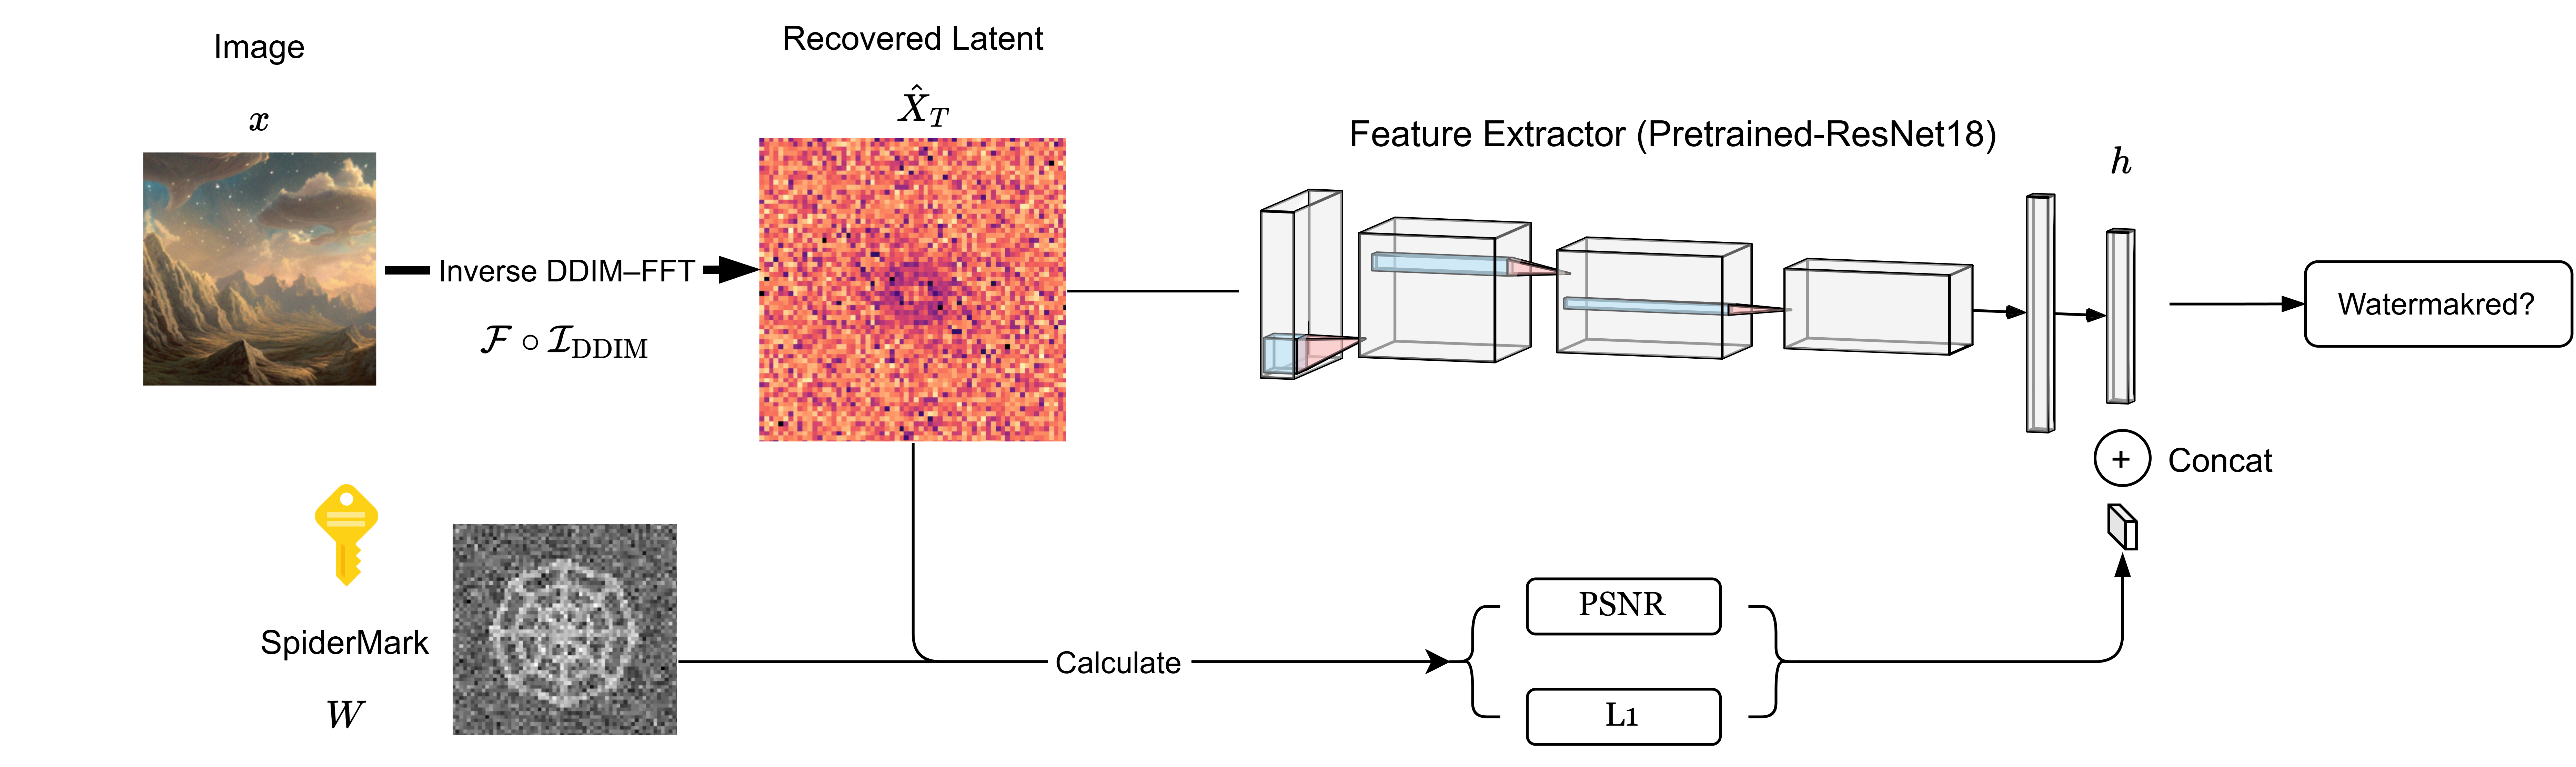
\includegraphics[width=1\linewidth]{figures/verifier_arch.png}
    \caption{{\color{blue}Verifier ($f_\theta$) Architecture. Given an input image, we first recover its corresponding watermark latent via inverse DDIM followed by a Fourier transform. The resulting frequency-domain representation is processed by a pretrained ResNet-18 verifier, augmented with auxiliary similarity cues (PSNR and L1) computed against the fixed SpiderMark pattern. The verifier outputs a probabilistic prediction indicating whether the image is watermarked.}}
    \label{fig:veifier_arch}
\end{figure*}


% \paragraph{Watermark Verification (Inference).}

% Given a query image $x$, SpiderMark determines the presence of the embedded watermark through a lightweight inference procedure that operates entirely in the frequency domain.
% Unlike injection and dataset construction, the verification stage does not require access to prompts, noise seeds, or the diffusion generator.

% For verification, we apply the inverse DDIM procedure corresponding to the same pretrained diffusion model used during generation.
% We treat inverse DDIM as a deterministic operator that approximately recovers the terminal latent noise from a generated image.
% Let $\mathcal{I}_{\text{DDIM}}(\cdot)$ denote this inverse mapping, and compute
% \begin{equation}
%     \hat{x}_T = \mathcal{I}_{\text{DDIM}}(x).
% \end{equation}

% The recovered latent $\hat{x}_T$ is transformed into the frequency domain via a two-dimensional Fourier transform,
% \begin{equation}
%     \hat{X}_T = \mathcal{F}\{\hat{x}_T\},
% \end{equation}
% where $(u,v)$ index the vertical and horizontal spatial-frequency components.
% We construct the verifier input as the magnitude spectrum
% \begin{equation}
%     S(u,v) = \left|\hat{F}_T(u,v)\right|,
% \end{equation}
% which captures the spectral footprint induced by watermark injection while discarding phase information that is less stable under image perturbations.

% Since SpiderMark embeds a fixed and known watermark pattern $W(u,v)$ during injection, we additionally compute explicit similarity measures between the recovered spectrum and the reference pattern.
% Specifically, we compute a masked $\ell_1$ distance
% \begin{equation}
%     d_{\ell_1} = \frac{1}{\|M\|_1} \left\| M \odot \left(S - W\right) \right\|_1,
% \end{equation}
% and a masked peak signal-to-noise ratio (PSNR),
% \begin{equation}
%     \mathrm{PSNR}_M = 10 \log_{10} \left( \frac{\mathrm{MAX}^2}{\mathrm{MSE}_M + \epsilon} \right),
% \end{equation}
% where
% \begin{equation}
%     \mathrm{MSE}_M = \frac{1}{\|M\|_1} \left\| M \odot \left(S - W\right) \right\|_2^2.
% \end{equation}
% Here, $M(u,v)$ denotes a binary mask defining the watermark support in the frequency domain, $\mathrm{MAX}$ is the maximum possible value of the normalized spectrum magnitude, and $\epsilon$ is a small constant for numerical stability.

% Finally, the magnitude spectrum $S(u,v)$ is processed by a convolutional backbone $\phi(\cdot)$ to extract deep frequency-domain features.
% The resulting feature embedding is concatenated with the two scalar similarity cues $(\mathrm{PSNR}_M, d_{\ell_1})$ and passed to a lightweight verifier head, which outputs a calibrated watermark confidence score $p \in [0,1]$.
% A binary verification decision is obtained by thresholding $p$ at a fixed operating point $\tau$.
% The complete inference procedure is summarised in Algorithm~\ref{alg:verification_inference}.


% \begin{algorithm}[t]
% \caption{Watermark Verification (Inference)}
% \label{alg:verification_inference}
% \begin{algorithmic}[1]
% \Require
% Query image $x$;
% inverse DDIM operator $\mathcal{I}_{\text{DDIM}}(\cdot)$;
% Fourier transform $\mathcal{F}(\cdot)$;
% reference watermark pattern $W$ and mask $M$;
% feature extractor $\phi(\cdot)$;
% trained verifier $f_\theta(\cdot)$;
% decision threshold $\tau$.

% \Ensure
% Watermark confidence $p \in [0,1]$;
% verification decision $\mathbb{1}[p \ge \tau]$.

% \State Recover terminal latent noise: $\hat{x}_T \leftarrow \mathcal{I}_{\text{DDIM}}(x)$.
% \State Compute spectrum magnitude: $S \leftarrow \left| \mathcal{F}\{\hat{x}_T\} \right|$.

% \State Compute masked $\ell_1$ similarity:
% \State \hspace{1.2em} $d_{\ell_1} \leftarrow \frac{1}{\|M\|_1} \left\| M \odot (S - W) \right\|_1$.
% \State Compute masked PSNR:
% \State \hspace{1.2em} $\mathrm{MSE}_M \leftarrow \frac{1}{\|M\|_1} \left\| M \odot (S - W) \right\|_2^2$.
% \State \hspace{1.2em} $\mathrm{PSNR}_M \leftarrow 10 \log_{10}\!\left(\frac{\mathrm{MAX}^2}{\mathrm{MSE}_M + \epsilon}\right)$.

% \State Extract deep features: $h \leftarrow \phi(S)$.
% \State Fuse cues and predict: $p \leftarrow f_\theta\!\left([h;\ \mathrm{PSNR}_M;\ d_{\ell_1}]\right)$.
% \State Output decision: $\mathbb{1}[p \ge \tau]$.
% \end{algorithmic}
% \end{algorithm}



{\color{blue}
\paragraph{Watermark Verification (Inference).}

Given a query image $x$, SpiderMark determines the presence of the embedded watermark through a lightweight inference procedure that operates in the frequency domain.
Unlike injection and dataset construction, the verification stage does not require access to prompts, noise seeds, or the diffusion generator.

For verification, we apply the inverse DDIM procedure corresponding to the same pretrained diffusion model and noise schedule used during generation.
We treat inverse DDIM as a deterministic operator that approximately recovers the terminal latent noise from a generated image.
Let $\mathcal{I}_{\text{DDIM}}(\cdot)$ denote this inverse mapping, and compute
\begin{equation}
    \hat{x}_T = \mathcal{I}_{\text{DDIM}}(x).
\end{equation}

The recovered latent $\hat{x}_T$ is transformed into the frequency domain via a two-dimensional Fourier transform,
\begin{equation}
    \hat{X}_T = \mathcal{F}\{\hat{x}_T\},
\end{equation}

Since SpiderMark embeds a fixed and known watermark pattern $W$ during injection, we additionally compute explicit similarity measures between the recovered spectrum and the reference pattern within the watermark support.
Let $M(u,v)$ denote a binary mask defining the watermark support in the frequency domain.
We compute a masked $\ell_1$ distance
\begin{equation}
    d_{\ell_1} = \frac{1}{\|M\|_1}\left\| M \odot \left(\hat{X}_T - W\right) \right\|_1,
\end{equation}
and a masked peak signal-to-noise ratio (PSNR),
\begin{equation}
    \mathrm{PSNR}_M = 10 \log_{10}\!\left( \frac{\mathrm{MAX}^2}{\mathrm{MSE}_M + \epsilon} \right),
\end{equation}
where
\begin{equation}
    \mathrm{MSE}_M = \frac{1}{\|M\|_1}\left\| M \odot \left(\hat{X}_T - W\right) \right\|_2^2.
\end{equation}
Here, $\mathrm{MAX}$ denotes the maximum possible value of the normalized real-valued representation of $\hat{X}_T$, and $\epsilon$ is a small constant for numerical stability.

Finally, the recovered spectrum $\hat{X}_T$ is processed by the verifier network $f_\theta(\cdot)$, which internally extracts deep frequency-features and fuses them with the two scalar similarity cues $(\mathrm{PSNR}_M, d_{\ell_1})$ in its final prediction layer.
Concretely, the backbone of $f_\theta$ produces an embedding $h$, which is concatenated with $(\mathrm{PSNR}_M, d_{\ell_1})$ and fed into the last layer to output a calibrated watermark confidence score $p \in [0,1]$.
A binary verification decision is obtained by thresholding $p$ at a fixed operating point $\tau$.
The complete inference procedure is summarised in Algorithm~\ref{alg:verification_inference}.

\begin{algorithm}[t]
\caption{Watermark Verification (Inference)}
\label{alg:verification_inference}
\begin{algorithmic}[1]
\Require
Query image $x$;
inverse DDIM operator $\mathcal{I}_{\text{DDIM}}(\cdot)$;
Fourier transform $\mathcal{F}\{\cdot\}$;
reference watermark pattern $W$ and mask $M$;
trained verifier $f_\theta(\cdot)$;
normalization constant $\mathrm{MAX}$;
stability constant $\epsilon$;
decision threshold $\tau$.

\Ensure
Watermark confidence $p \in [0,1]$;
verification decision $\mathbb{1}[p \ge \tau]$.

\State Recover terminal latent noise: $\hat{x}_T \leftarrow \mathcal{I}_{\text{DDIM}}(x)$.
\State Compute Fourier spectrum: $\hat{X}_T \leftarrow \mathcal{F}\{\hat{x}_T\}$.

\State Compute masked $\ell_1$ similarity:
\State \hspace{1.2em} $d_{\ell_1} \leftarrow \frac{1}{\|M\|_1}\left\| M \odot (\hat{X}_T - W) \right\|_1$.
\State Compute masked PSNR:
\State \hspace{1.2em} $\mathrm{MSE}_M \leftarrow \frac{1}{\|M\|_1}\left\| M \odot (\hat{X}_T - W) \right\|_2^2$.
\State \hspace{1.2em} $\mathrm{PSNR}_M \leftarrow 10 \log_{10}\!\left(\frac{\mathrm{MAX}^2}{\mathrm{MSE}_M + \epsilon}\right)$.

\State Predict watermark confidence (fusion occurs in the last layer of $f_\theta$):
\State \hspace{1.2em} $p \leftarrow f_\theta(\hat{X}_T, \mathrm{PSNR}_M, d_{\ell_1})$.
\State Output decision: $\mathbb{1}[p \ge \tau]$.
\end{algorithmic}
\end{algorithm}
}
\section{Results}

\subsection{Experimental Setup}
SpiderMark is evaluated on a diverse suite of image perturbations to assess watermark detectability and robustness under real-world transformations. 
Experiments are conducted using a Stable Diffusion v2.1 backbone, where the watermark is injected into the initial noise tensor \(x_T\). 
The verification model is trained to classify between watermarked and non-watermarked images in the frequency domain, while a PSNR-based detector with a fixed sigmoid threshold of \(-4\) serves as the baseline.

Nine types of image transformations are applied:  
(1) \textit{clean}, (2) \textit{jpeg\_strong}, (3) \textit{msg\_app\_combo}, (4) \textit{down\_up}, (5) \textit{blur}, (6) \textit{random\_crop}, (7) \textit{occlusion}, (8) \textit{geom\_warp}, and (9) \textit{train\_aug\_mix}.  
These augmentations simulate practical degradations such as compression, scaling, occlusion, and geometric distortion commonly seen in content sharing platforms.


\paragraph{Verifier Training Details.}
We sample prompts from the public \texttt{Gustavosta/Stable-Diffusion-Prompts} collection and generate a balanced dataset of 500 watermarked and 500 non-watermarked images using Stable Diffusion v2.1.
All images are converted to grayscale, transformed using a 2D FFT, and the magnitude spectrum is provided to a ResNet-18 verifier pretrained on ImageNet.
The model is fine-tuned using binary cross-entropy loss.

% %%% TODO: 5x5 matrix - find 5 examples and show the five algorithms
% \begin{figure*}[t]
%     \centering

%     % ---- Row 1 ----
%     \begin{subfigure}[b]{0.31\linewidth}
%         \centering
%         
\includegraphics[width=\linewidth]{clean_image.png}
%         \caption{Clean Image}
%     \end{subfigure}
%     \hfill
%     \begin{subfigure}[b]{0.31\linewidth}
%         \centering
%         
\includegraphics[width=\linewidth]{spidernet_watermarked.png}
%         \caption{SpiderMark Watermark}
%     \end{subfigure}
%     \hfill
%     \begin{subfigure}[b]{0.31\linewidth}
%         \centering
%         
\includegraphics[width=\linewidth]{ring_watermarked.png}
%         \caption{Ring Watermarked}
%     \end{subfigure}

%     \vspace{6mm}

%     % ---- Row 2 ----
%     \begin{subfigure}[b]{0.49\linewidth}
%         \centering
%         
\includegraphics[width=0.62\linewidth]{dft_single_str10.PNG}
%         \caption{DFT-Single Watermark}
%     \end{subfigure}
%     \hfill
%     \begin{subfigure}[b]{0.49\linewidth}
%         \centering
%         
\includegraphics[width=0.62\linewidth]{dwtdct_alpha0_5.PNG}
%         \caption{DWT-DCT Watermark}
%     \end{subfigure}

%     \caption{Visual comparison of different watermarking methods.}
%     \label{fig:watermark_comparison}
% \end{figure*}

\begin{figure*}[t]
    \centering

    % ---------- Row 1: Clean ----------
    \begin{subfigure}[t]{0.19\textwidth}
        
\includegraphics[width=\linewidth]{figures/paper_grid/clean/0000.png}
    \end{subfigure}
    \begin{subfigure}[t]{0.19\textwidth}
        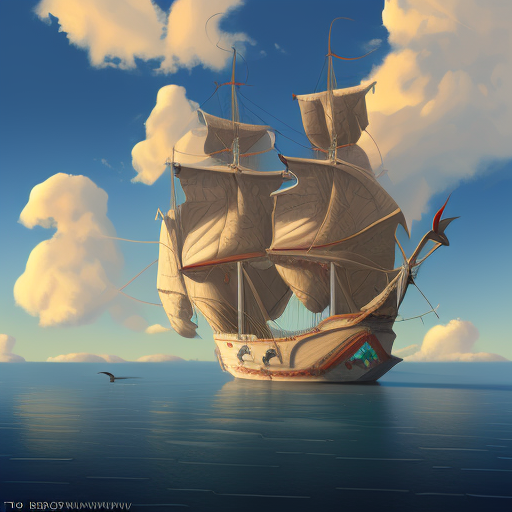
\includegraphics[width=\linewidth]{figures/paper_grid/clean/0002.png}
    \end{subfigure}
    \begin{subfigure}[t]{0.19\textwidth}
        
\includegraphics[width=\linewidth]{figures/paper_grid/clean/0004.png}
    \end{subfigure}
    \begin{subfigure}[t]{0.19\textwidth}
        
\includegraphics[width=\linewidth]{figures/paper_grid/clean/0016.png}
    \end{subfigure}
    \begin{subfigure}[t]{0.19\textwidth}
        
\includegraphics[width=\linewidth]{figures/paper_grid/clean/0021.png}
    \end{subfigure}

    \vspace{2mm}

    % ---------- Row 4: Our ----------
    \begin{subfigure}[t]{0.19\textwidth}
        
\includegraphics[width=\linewidth]{figures/paper_grid/our/0000.png}
    \end{subfigure}
    \begin{subfigure}[t]{0.19\textwidth}
        
\includegraphics[width=\linewidth]{figures/paper_grid/our/0002.png}
    \end{subfigure}
    \begin{subfigure}[t]{0.19\textwidth}
        
\includegraphics[width=\linewidth]{figures/paper_grid/our/0004.png}
    \end{subfigure}
    \begin{subfigure}[t]{0.19\textwidth}
        
\includegraphics[width=\linewidth]{figures/paper_grid/our/0016.png}
    \end{subfigure}
    \begin{subfigure}[t]{0.19\textwidth}
        
\includegraphics[width=\linewidth]{figures/paper_grid/our/0021.png}
    \end{subfigure}

    \vspace{2mm}

    % ---------- Row 5: Tree-Ring ----------
    \begin{subfigure}[t]{0.19\textwidth}
        
\includegraphics[width=\linewidth]{figures/paper_grid/tree-ring/0000.png}
    \end{subfigure}
    \begin{subfigure}[t]{0.19\textwidth}
        
\includegraphics[width=\linewidth]{figures/paper_grid/tree-ring/0002.png}
    \end{subfigure}
    \begin{subfigure}[t]{0.19\textwidth}
        
\includegraphics[width=\linewidth]{figures/paper_grid/tree-ring/0004.png}
    \end{subfigure}
    \begin{subfigure}[t]{0.19\textwidth}
        
\includegraphics[width=\linewidth]{figures/paper_grid/tree-ring/0016.png}
    \end{subfigure}
    \begin{subfigure}[t]{0.19\textwidth}
        
\includegraphics[width=\linewidth]{figures/paper_grid/tree-ring/0021.png}
    \end{subfigure}

    % ---------- Row 2: DFT ----------
    \begin{subfigure}[t]{0.19\textwidth}
        
\includegraphics[width=\linewidth]{figures/paper_grid/dft/0000_wm.png}
    \end{subfigure}
    \begin{subfigure}[t]{0.19\textwidth}
        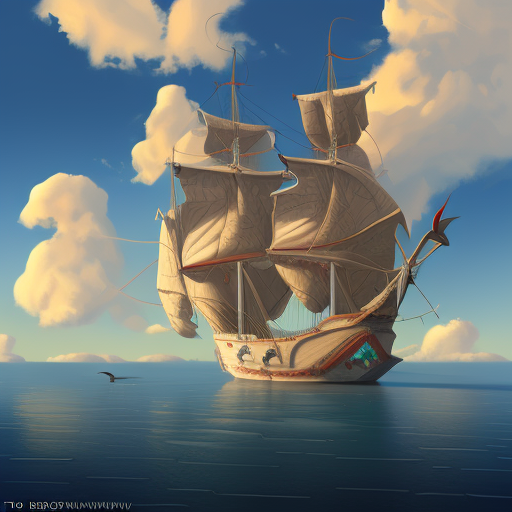
\includegraphics[width=\linewidth]{figures/paper_grid/dft/0002_wm.png}
    \end{subfigure}
    \begin{subfigure}[t]{0.19\textwidth}
        
\includegraphics[width=\linewidth]{figures/paper_grid/dft/0004_wm.png}
    \end{subfigure}
    \begin{subfigure}[t]{0.19\textwidth}
        
\includegraphics[width=\linewidth]{figures/paper_grid/dft/0016_wm.png}
    \end{subfigure}
    \begin{subfigure}[t]{0.19\textwidth}
        
\includegraphics[width=\linewidth]{figures/paper_grid/dft/0021_wm.png}
    \end{subfigure}

    \vspace{2mm}

    % ---------- Row 3: DWT ----------
    \begin{subfigure}[t]{0.19\textwidth}
        
\includegraphics[width=\linewidth]{figures/paper_grid/dwt/0000_wm.png}
    \end{subfigure}
    \begin{subfigure}[t]{0.19\textwidth}
        
\includegraphics[width=\linewidth]{figures/paper_grid/dwt/0002_wm.png}
    \end{subfigure}
    \begin{subfigure}[t]{0.19\textwidth}
        
\includegraphics[width=\linewidth]{figures/paper_grid/dwt/0004_wm.png}
    \end{subfigure}
    \begin{subfigure}[t]{0.19\textwidth}
        
\includegraphics[width=\linewidth]{figures/paper_grid/dwt/0016_wm.png}
    \end{subfigure}
    \begin{subfigure}[t]{0.19\textwidth}
        
\includegraphics[width=\linewidth]{figures/paper_grid/dwt/0021_wm.png}
    \end{subfigure}

    \vspace{2mm}
    \caption{
    Visual comparison across watermarking methods.
    Rows correspond to Clean, Our method, Tree-Ring, DFT and DWT.
    Columns show different image instances.
    }
    \label{fig:watermark_grid}
\end{figure*}


\paragraph{Robustness Evaluation.}
SpiderMark is evaluated under a comprehensive set of post-processing transformations that simulate real-world image distortions. 
Each perturbation is applied to generated images before verification, and both the SpiderMark detector and PSNR baseline (threshold = -4) are evaluated over five independent runs to obtain averaged values. 
The following perturbations are considered:
\begin{itemize}
    \item \textit{Clean}: unmodified images as a reference.
    \item \textit{JPEG-Strong}: aggressive JPEG compression at low quality.
    \item \textit{MsgApp-Combo}: chained resampling and recompression to emulate messaging app transmission.
    \item \textit{Down-Up}: downsampling followed by upsampling to simulate resolution scaling.
    \item \textit{Blur}: Gaussian blur representing optical or motion blur.
    \item \textit{Random Crop}: random resized crops reflecting framing changes.
    \item \textit{Occlusion}: partial masking to assess redundancy and spatial resilience.
    \item \textit{Geom-Warp}: geometric warping and affine distortion.
    \item \textit{Aug-Mix}: composite augmentations used to test generalisation.
\end{itemize}
Evaluation metrics include accuracy and AUROC, averaged across all trials.

\subsection{Quantitative Evaluation}

\begin{table*}[h]
\centering
\caption{Watermark verification performance under various image transformations.
The learned detector (with or without the pattern and mask, PM) is compared against classical
Tree-Ring verification methods \citep{wen2023treeringwatermarksfingerprintsdiffusion}, along with the DFT-Single and DWT-DCT frequency
watermarking baselines. Bold values indicate row-wise best performance. As discussed in
Section~\ref{subsec:auc_limitations}, accuracy at a fixed threshold provides a more reliable
measure of robustness than AUC, since AUC can remain high even when the optimal threshold
varies significantly across different distortions.}
\label{tab:robustness_results_all}
\resizebox{\textwidth}{!}{
\begin{tabular}{lcccccccccc}
\toprule
\multirow{2}{*}{\textbf{Attack}} &
\multicolumn{2}{c}{\textbf{Ours (+PL)}} &
\multicolumn{2}{c}{\textbf{Ours (-PL)}} &
\multicolumn{2}{c}{\textbf{Tree-Ring}} &
\multicolumn{2}{c}{\textbf{DFT-Single}} &
\multicolumn{2}{c}{\textbf{DWT--DCT}} \\
\cmidrule(lr){2-3}
\cmidrule(lr){4-5}
\cmidrule(lr){6-7}
\cmidrule(lr){8-9}
\cmidrule(lr){10-11}
& Acc & AUROC
& Acc & AUROC
& Acc & AUROC
& Acc & AUROC
& Acc & AUROC \\
\midrule

clean           
& \underline{0.9467} & \underline{0.9904}
& 0.8533 & 0.9848
& \textbf{0.9759} & \textbf{0.9971}  
& 0.9090 & 0.9603
& 0.6760 & 0.7199
\\

jpeg\_strong    
& \textbf{0.8720} & \textbf{0.9410}
& \underline{0.7253} & 0.8164
& 0.6627 & \underline{}{0.8772}
& 0.5717 & 0.5730
& 0.6737 & 0.7156
\\

msg\_app\_combo 
& \textbf{0.6813} & \textbf{0.8468}
& 0.5733 & 0.6527
& 0.4747 & \underline{0.8136}
& 0.5223 & 0.5044
& \underline{0.6700} & 0.7113
\\

down\_up        
& \textbf{0.9133} & \textbf{0.9713}
& \underline{0.7600} & 0.8461
& 0.6988 & \underline{0.9576}
& 0.5270 & 0.5164
& 0.6720 & 0.7159
\\

blur            
& \textbf{0.8160} & \textbf{0.8757}
& 0.6427 & 0.6896
& 0.4771 & \underline{0.7777}
& 0.5620 & 0.5717
& \underline{0.6690} & 0.7103
\\

random\_crop    
& \textbf{0.8787} & \underline{0.9503}
& \underline{0.8373} & 0.9102
& 0.7807 & \textbf{0.9565}
& 0.5133 & 0.4912
& 0.5220 & 0.5046
\\

occlusion       
& \textbf{0.9574} & \underline{0.9878}
& 0.9067 & 0.9721
& \underline{0.9325} & \textbf{0.9915}
& 0.9080 & 0.9582
& 0.6603 & 0.6939
\\

geom\_warp      
& \textbf{0.8560} & \underline{0.9381}
& \underline{0.7893} & 0.8734
& 0.7711 & \textbf{0.9412}
& 0.5190 & 0.4909
& 0.5193 & 0.5083
\\

train\_aug\_mix 
& \underline{0.7280} & \underline{0.8620}
& \textbf{0.7400} & 0.8242 
& 0.6337 & \textbf{0.8634}
& 0.5417 & 0.5340
& 0.5360 & 0.5283
\\

\bottomrule
\end{tabular}

}
\end{table*}





\begin{table}[h!]
\centering
\begin{tabular}{lcc}
\hline
\textbf{Attack} & \textbf{Best L1 Thr} & \textbf{Best PSNR Thr} \\
\hline
clean          & -78.2500  & 5.3937 \\
jpeg\_strong   & -82.2500  & 4.9414 \\
msg\_app\_combo & -87.3750  & 4.3452 \\
down\_up       & -82.5625  & 4.6217 \\
blur           & -83.8750  & 4.0488 \\
random\_crop   & -82.6875  & 5.0281 \\
occlusion      & -79.9375  & 5.2857 \\
geom\_warp     & -81.0625  & 5.2801 \\
train\_aug\_mix & -82.1875 & 4.9464 \\
\hline
\end{tabular}
\caption{Optimal thresholds for L1 and PSNR detectors under different attacks. Large threshold shifts indicate that AUC alone is unreliable for evaluating watermark detection robustness.}
\label{tab:threshold_shift}
\end{table}


Across all attack scenarios, SpiderMark achieves significantly higher accuracy and AUROC than the PSNR baseline.  
While PSNR quickly loses discriminative power under pixel-level corruptions, the learned detector maintains reliable separability (AUROC \(>\) 0.7–0.9) even under strong distortions such as compression, blur, or warping.  
Both detectors perform comparably on clean images, confirming that SpiderMark does not compromise the fidelity of unperturbed outputs.

\subsection{Evaluation on COCO Dataset}

To evaluate cross-dataset generalisation, we further assess watermark verification performance on the COCO dataset, which is not used during verifier training. In contrast to prior experiments where the verifier is trained and evaluated on images generated from the Stable Diffusion prompt dataset, this setting tests whether the learned verifier overfits to prompt distributions or generation characteristics seen during training.

Table~\ref{tab:coco_four_methods} reports verification performance under a range of common signal-processing and geometric distortions. Despite being trained solely on Stable Diffusion prompts, our method (SpiderMark) consistently achieves the highest accuracy and AUROC across nearly all attack types on COCO. This includes challenging transformations such as strong JPEG compression, random cropping, geometric warping, and mixed training-time augmentations.

Notably, the performance gap between SpiderMark and prior methods remains substantial even under severe distortions. Tree-Ring shows moderate degradation when transferring to COCO, while frequency-based baselines such as DFT-Single and DWT--DCT exhibit significant performance drops, particularly under geometric and mixed attacks. These results indicate that our verifier does not rely on dataset-specific artifacts, but instead learns watermark-consistent frequency-domain cues that generalise across datasets.

Importantly, this generalisation is achieved without retraining or fine-tuning the verifier on COCO, highlighting the robustness of the proposed verification strategy under distribution shift. Furthermore, FID scores reported in the last row indicate that SpiderMark maintains comparable image quality to other watermarking methods, suggesting that improved robustness does not come at the cost of perceptual degradation.

Overall, these results demonstrate that the proposed watermarking and verification framework generalises effectively to unseen datasets, reinforcing its practicality for real-world deployment where training and test distributions may differ substantially.


\begin{table*}[h]
\centering
\caption{Watermark verification performance on COCO (unseen dataset) under various image transformations.
FID scores are shown as a separate row for each watermarking method.}
\label{tab:coco_four_methods}

\resizebox{.8\textwidth}{!}{
\begin{tabular}{lcccccccc}
\toprule
\multirow{2}{*}{\textbf{Attack / Metric}} &

\multicolumn{2}{c}{\textbf{SpiderMark}} &
\multicolumn{2}{c}{\textbf{Tree-Ring}} &
\multicolumn{2}{c}{\textbf{DFT-Single}} &
\multicolumn{2}{c}{\textbf{DWT--DCT}} \\

\cmidrule(lr){2-3}
\cmidrule(lr){4-5}
\cmidrule(lr){6-7}
\cmidrule(lr){8-9}

& Acc & AUROC
& Acc & AUROC
& Acc & AUROC
& Acc & AUROC \\
\midrule

clean           
& \textbf{0.9733} & \textbf{0.9925}
& 0.8800 & 0.9483
& 0.8840 & 0.9433
& 0.6630 & 0.7062
\\

jpeg\_strong    
& \textbf{0.9000} & \textbf{0.9735}
& 0.7987 & 0.8800
& 0.5793 & 0.5934
& 0.6590 & 0.7009
\\

msg\_app\_combo 
& \textbf{0.7733} & \textbf{0.8820}
& 0.6360 & 0.7556
& 0.5240 & 0.5106
& 0.6567 & 0.6972
\\

down\_up        
& \textbf{0.9133} & \textbf{0.9720}
& 0.7800 & 0.8992
& 0.5130 & 0.4996
& 0.6600 & 0.7026
\\

blur            
& \textbf{0.8173} & \textbf{0.8877}
& 0.6440 & 0.7694
& 0.5540 & 0.5469
& 0.6557 & 0.6975
\\

random\_crop    
& \textbf{0.8240} & \textbf{0.9169}
& 0.7413 & 0.8451
& 0.5177 & 0.4973
& 0.5180 & 0.5011
\\

occlusion       
& \textbf{0.9720} & \textbf{0.9908}
& 0.8560 & 0.9398
& 0.8820 & 0.9402
& 0.6417 & 0.6832
\\

geom\_warp      
& \textbf{0.8373} & \textbf{0.9300}
& 0.7613 & 0.8377
& 0.5147 & 0.4871
& 0.5317 & 0.5173
\\

train\_aug\_mix 
& \textbf{0.7227} & \textbf{0.8389}
& 0.6813 & 0.7730
& 0.5360 & 0.5330
& 0.5360 & 0.5325
\\

\midrule\midrule
FID score  (non-watermarked = 81.743)
& \multicolumn{2}{c}{\underline{83.2103}}
& \multicolumn{2}{c}{83.5059}
& \multicolumn{2}{c}{\textbf{81.7612}}
& \multicolumn{2}{c}{83.3128} \\
\bottomrule

\end{tabular}
}
\end{table*}





\subsection{Semantic Preservation Evaluation using CLIP}

\begin{table}[t]
\centering
\caption{CLIP image--text semantic similarity comparison between clean (unwatermarked) images and different watermarking methods. Higher values indicate better semantic alignment.}
\label{tab:clip_similarity}
\begin{tabular}{lcc}
\toprule
\textbf{Method} & \textbf{COCO} & \textbf{Stable Diffusion} \\
\midrule
Unwatermarked & \textbf{0.3302} & \textbf{0.3615} \\
Tree-Ring             & 0.3296          & 0.3614          \\
Ours (Spidermark)        & 0.3273          & 0.3599          \\
\bottomrule
\end{tabular}
\end{table}


To assess whether watermark injection alters the semantic content of generated images, we evaluate image--text semantic similarity using CLIP. For each image, we compute the cosine similarity between the CLIP image embedding and its corresponding generation prompt. We report the mean CLIP similarity over all samples, with higher values indicating better semantic alignment.

Table~\ref{tab:clip_similarity} presents results on both the COCO and Stable Diffusion verification datasets. Clean (unwatermarked) images achieve mean CLIP similarities of 0.3302 and 0.3615 on COCO and Stable Diffusion, respectively. Tree-Ring produces nearly identical scores, indicating minimal semantic distortion. Our method (OctoWeb) achieves CLIP similarities of 0.3273 on COCO and 0.3599 on Stable Diffusion.

Notably, the semantic gap between our method and clean images is extremely small (no more than 0.003 across both datasets), which is well below commonly accepted thresholds for significant semantic degradation. This demonstrates that the proposed watermarking strategy preserves the semantic alignment between images and their prompts while remaining comparable to state-of-the-art frequency-domain watermarking methods.

Overall, these results confirm that the proposed approach introduces negligible semantic distortion, maintaining high fidelity to the original prompt semantics across different datasets.


\subsection{Ablation — Without Watermark Pattern and Mask for Verification Model}

To evaluate the contribution of the watermark pattern and mask as auxiliary inputs to the verification model, 
we conducted an ablation experiment by removing both components during inference and retraining the model 
under identical conditions. The goal of this analysis is to determine whether the inclusion of watermark-related inputs provides measurable robustness improvements under various image transformations.

Table~\ref{tab:robustness_results_all} compares the performance between the +PL model (with PSNR \& L1), its ablated counterpart,-PL (without PSNR \& L1). 
Across most transformation types, the model +PL achieves higher or comparable accuracy 
and AUROC, particularly under \textit{clean}, \textit{down\_up}, and \textit{occlusion} conditions. The improvements are most pronounced in scenarios where structural or frequency-domain cues from the watermark pattern enhance detection stability against geometric and photometric distortions.

In contrast, the model without the watermark and mask shows slightly lower robustness to severe degradations such as \textit{jpeg\_strong} and \textit{blur}, suggesting that these auxiliary inputs help preserve feature consistency under compression and noise. Nevertheless, both versions maintain a significant advantage over the PSNR baseline, confirming the effectiveness of the learned detector architecture. 
Overall, this ablation study demonstrates that the watermark pattern and mask provide complementary cues that improve verification reliability under challenging transformations.

\section{Discussion}

This section synthesises the experimental findings and discusses their implications for practical watermark verification in diffusion-based generative models, with particular emphasis on robustness, generalisation, and deployment-oriented evaluation.

\subsection{Overall Robustness of the Learned Detector}

The results consistently demonstrate that SpiderMark achieves strong and stable watermark verification across a wide range of photometric, geometric, and mixed distortions. Unlike handcrafted similarity metrics, the learned verifier maintains reliable performance even under aggressive transformations such as strong JPEG compression, spatial resampling, and partial occlusion.

Importantly, the detector’s robustness extends beyond pixel-level fidelity. The sustained performance under spatial misalignment and local corruption suggests that the watermark signal is encoded in structured frequency-domain patterns that propagate through the diffusion process and remain detectable after substantial post-processing. This confirms that the proposed injection strategy produces a watermark that is both imperceptible and structurally persistent, while the learned verifier effectively captures these stable cues.

\subsection{Limitations of AUC as a Robustness Metric}\label{subsec:auc_limitations}


\begin{figure*}
    \centering
    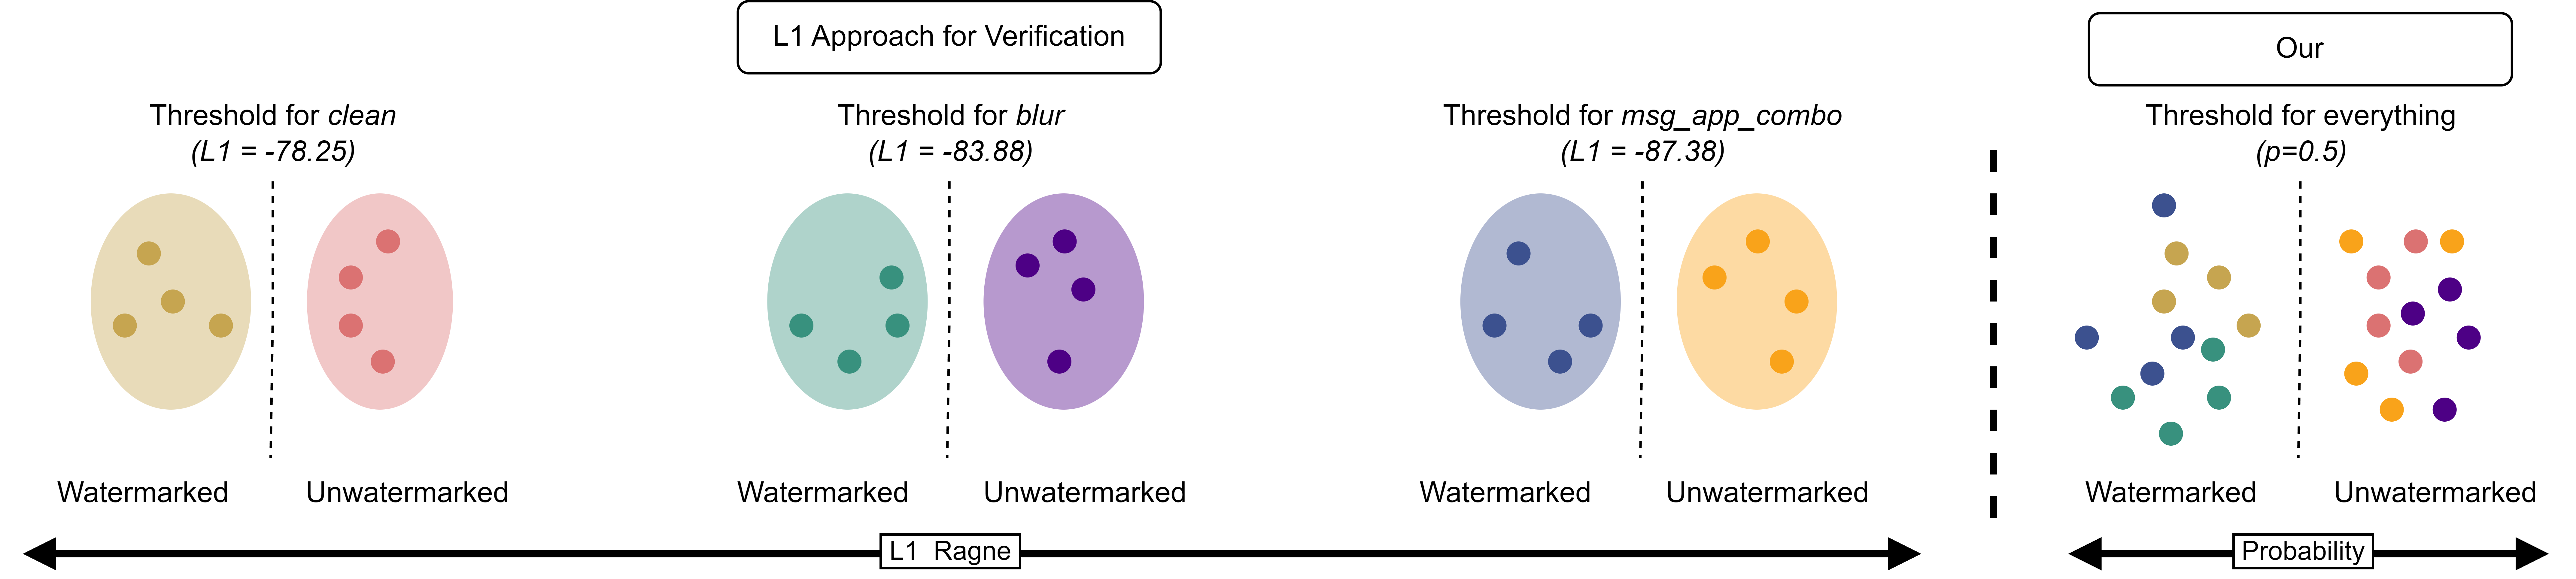
\includegraphics[width=1\linewidth]{figures/l1_not_best.png}
    \caption{Conceptual comparison between L1-distance--based verification and our probabilistic verification approach. 
        \textbf{Left:} Under different attacks, the distributions of L1 distances for watermarked and unwatermarked images shift in an attack-dependent manner, resulting in no single universal decision threshold.
        \textbf{Right:} Our method maps verification evidence to calibrated probabilities, enabling more stable and attack-invariant decision-making without relying on a fixed distance threshold.}
    \label{fig:l1_limitations}
\end{figure*}



Although AUROC is a common metric for evaluating binary classifiers, our experiments highlight its limitations for assessing watermark robustness in real-world deployment scenarios. In practice, watermark verification systems must operate at a \emph{fixed decision threshold}, whereas AUROC evaluates separability by sweeping over all possible thresholds. As a result, a high AUROC does not necessarily translate into reliable verification performance at inference time.

As shown in Table~\ref{tab:threshold_shift}, the optimal thresholds for distance-based detectors such as L1 or PSNR vary substantially across different attack types. This threshold instability persists even when AUROC remains high, indicating that separability alone is insufficient to guarantee robustness under unknown or mixed distortions.

Figure~\ref{fig:l1_limitations} provides an intuitive illustration of this phenomenon. Scalar distance metrics induce attack-dependent shifts in score distributions, making it impossible to select a single universal threshold. In contrast, the proposed verifier maps frequency-domain evidence to calibrated probabilities, enabling more stable decision-making under a fixed operating point. This probabilistic formulation is therefore better aligned with real-world deployment constraints.

\subsection{Photometric Robustness}

Under photometric degradations such as strong JPEG compression and Gaussian blur, SpiderMark substantially outperforms PSNR-based verification, which collapses to near-random performance. The resilience of the learned detector indicates that it leverages mid-frequency spectral structures that survive quantisation and smoothing, rather than relying on fragile pixel-level statistics.

This robustness is particularly important in real-world content distribution pipelines, where images are routinely re-encoded, resized, or compressed by platforms beyond the control of the content creator or verifier.

\subsection{Geometric and Spatial Robustness}

Spatial transformations such as downsampling–upsampling, geometric warping, and random cropping pose significant challenges for watermark verification due to spatial misalignment. Despite these distortions, SpiderMark maintains strong AUROC and accuracy, demonstrating that the verifier learns geometry-invariant watermark signatures in the frequency domain.

In contrast, classical baselines that depend on pixel alignment or fixed spatial correspondence degrade sharply once spatial consistency is disrupted. These results highlight the advantage of combining noise-level frequency injection with learned verification over rigid, handcrafted detection rules.

\subsection{Effect of Watermark Pattern and Mask (PM) Ablation}

The ablation study reveals that providing the watermark pattern and mask as auxiliary inputs generally improves verification robustness, particularly under compression, occlusion, and resampling. These components act as structural priors, guiding the verifier toward watermark-relevant spectral regions.

However, under severe geometric distortions such as random cropping, the spatial alignment between the pattern and the observed image may be compromised, reducing the benefit of explicit pattern conditioning. In such cases, the PM-agnostic model performs comparably, suggesting that augmentation-aware training could further enhance robustness when strong spatial perturbations are expected.

\subsection{Cross-Dataset Generalisation}

A key finding of this work is the strong generalisation of the verifier to unseen data distributions. Although the verifier is trained exclusively on images generated from the Stable Diffusion prompt dataset, it consistently achieves the best performance on the COCO dataset without any retraining or fine-tuning.

This result indicates that the verifier does not overfit to prompt-specific semantics or dataset-specific artefacts, but instead learns watermark-consistent frequency-domain cues that transfer across datasets. Such generalisation is essential for practical deployment, where the verifier may encounter images generated under diverse prompts, styles, or downstream usage contexts.

\subsection{Semantic Preservation and Perceptual Quality}

The CLIP-based semantic evaluation further confirms that SpiderMark introduces negligible semantic distortion. The observed differences in CLIP similarity between watermarked and unwatermarked images are consistently below 0.003 across both Stable Diffusion and COCO datasets, which is well below commonly accepted thresholds for perceptual or semantic degradation.

In conjunction with comparable FID scores, these results demonstrate that improved robustness does not come at the expense of image quality or semantic fidelity, reinforcing the practicality of the proposed approach.

\subsection{Implications for Real-World Deployment}

Taken together, these findings establish SpiderMark as a practical and deployment-ready watermarking framework for diffusion-based generative models. By combining noise-level frequency injection with probabilistic, threshold-aware verification, the proposed system addresses key limitations of existing watermarking approaches, including threshold instability, poor robustness under transformation, and limited generalisation.

The analysis also highlights the importance of evaluation protocols that reflect real-world operating constraints. Metrics that account for fixed thresholds and calibrated confidence scores provide a more faithful assessment of robustness than threshold-free measures such as AUROC alone. These insights are broadly applicable beyond watermarking and may inform the evaluation of other content attribution and authenticity systems.

\section{Conclusion}

This paper introduced \textit{SpiderMark}, a structured watermarking framework for diffusion-based image generation that embeds a fixed geometric pattern directly into the noise initialization stage in the frequency domain. Unlike prior approaches that rely on handcrafted similarity metrics or rigid frequency ring structures, SpiderMark unifies watermark injection and probabilistic verification into a single framework that remains fully compatible with pretrained diffusion models and does not require modifying model weights.

Extensive evaluations demonstrate that the proposed verifier substantially outperforms PSNR-based detection across a wide range of photometric, geometric, and mixed distortions. By learning watermark-consistent frequency cues rather than relying on pixel-level alignment, SpiderMark maintains reliable performance under compression, resampling, occlusion, and spatial warping. Ablation studies further show that conditioning the verifier on the watermark pattern and mask improves robustness in most settings while preserving image quality.

Crucially, the verifier generalises effectively beyond its training distribution. Despite being trained solely on images generated from the Stable Diffusion prompt dataset, SpiderMark achieves strong verification performance on the unseen COCO dataset without retraining, indicating that the learned features are not dataset- or prompt-specific. Semantic evaluation using CLIP similarity and perceptual assessment via FID confirm that watermark robustness is achieved without compromising image quality or semantic fidelity.

Beyond empirical performance, this work highlights important evaluation considerations for practical watermarking systems. In particular, we demonstrate that threshold-free metrics such as AUROC can be misleading under deployment constraints, and that calibrated, threshold-aware verification provides a more reliable measure of real-world robustness.

Overall, SpiderMark provides a practical and generalisable solution for content attribution in diffusion-based generative models. Future work may extend this framework to multimodal generation pipelines, investigate adaptive or content-aware watermarking strategies, and explore robustness against more extreme geometric or adversarial transformations.


{
    \small
    \bibliographystyle{ieeenat_fullname}
    \bibliography{main}
}

% WARNING: do not forget to delete the supplementary pages from your submission 
% \input{sec/X_suppl}

\end{document}
